%
\documentclass[dvipdfmx,11pt,notheorems]{beamer}
%%%% 和文用 %%%%%
\usepackage{bxdpx-beamer}
\usepackage{pxjahyper}
\usepackage{minijs}%和文用
\usepackage{hyperref}
\renewcommand{\kanjifamilydefault}{\gtdefault}%和文用に

%%%% スライドの見た目 %%%%%
\usetheme{Madrid}
\usefonttheme{professionalfonts}
\setbeamertemplate{frametitle}[default][center]
\setbeamertemplate{navigation symbols}{}
\setbeamercovered{transparent}%好みに応じてどうぞ)
\setbeamertemplate{footline}[page number]
\setbeamerfont{footline}{size=\normalsize,series=\bfseries}
\setbeamercolor{footline}{fg=black,bg=black}
\pagestyle{empty}
%%%%

%%%% 定義環境 %%%%%
\usepackage{amsmath,amssymb}
\usepackage{amsthm}
\usepackage{verbatim}
\theoremstyle{definition}
\newtheorem{theorem}{定理}
\newtheorem{definition}{定義}
\newtheorem{proposition}{命題}
\newtheorem{lemma}{補題}
\newtheorem{corollary}{系}
\newtheorem{conjecture}{予想}
\newtheorem*{remark}{Remark}
\renewcommand{\proofname}{}
%%%%%%%%%

%%%%% フォント基本設定 %%%%%
\usepackage[T1]{fontenc}%8bit フォント
\usepackage{textcomp}%欧文フォントの追加
\usepackage[utf8]{inputenc}%文字コードをUTF-8
\usepackage{otf}%otfパッケージ
\usepackage{lxfonts}%数式・英文ローマン体を Lxfont にする
\usepackage{bm}%数式太字にほんごにほんご
%%%%%%%%%%

\usefonttheme{professionalfonts}

\title[タイトル]{ニューラルネットワークで巡回セールスマン問題を解く}
\institute[JPN]{名古屋大学多元数理科学研究科}
\author[]{藤本勇希}
\date{2016/04/21}

\begin{document}

\begin{frame}[plain]\frametitle{}
\titlepage %表紙
\end{frame}

%\begin{frame}\frametitle{Contents}
%\tableofcontents %目次
%\end{frame}

%\section{巡回セールスマン問題}

\begin{frame}\frametitle{ニューラルネットワークとは}
人間の脳の働きの一部を模倣することにより、知的な情報処理の実現を目
指したものである。
\begin{center}
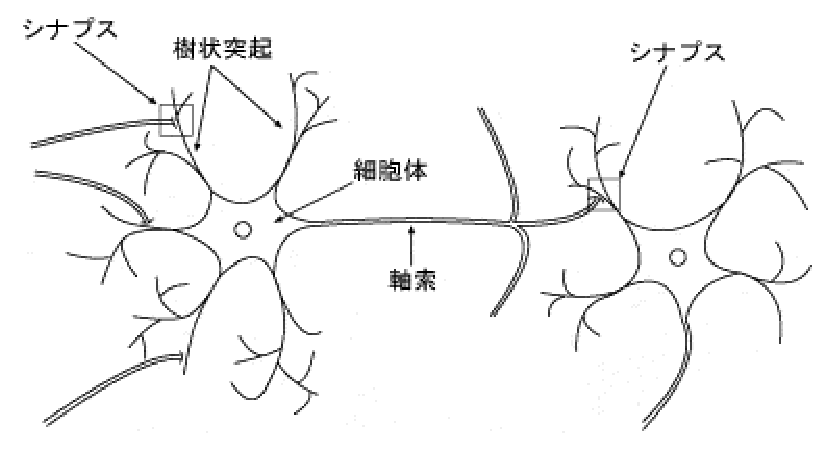
\includegraphics[width=6cm, height=4cm]{neuron.eps}
\end{center}
各ニューロンは、他のニューロンの出力をシナプスの強さに応じて入力として受け取り、その入力に応じて発火するかどうか決定する。
\end{frame}

\begin{frame}\frametitle{ニューロンのモデル}
ニューロンの発火のモデルは様々なものがあるが、出力がデジタルかアナログかで分類できる。
\begin{columns}[T]		
\begin{column}[T]{5cm}
\begin{figure}[htbp]
	\includegraphics[height=4cm, width=6cm]{gain.png}
	\caption{アナログ出力モデル}
\end{figure}
\end{column}
\begin{column}[T]{5cm}
\begin{figure}[htbp]
	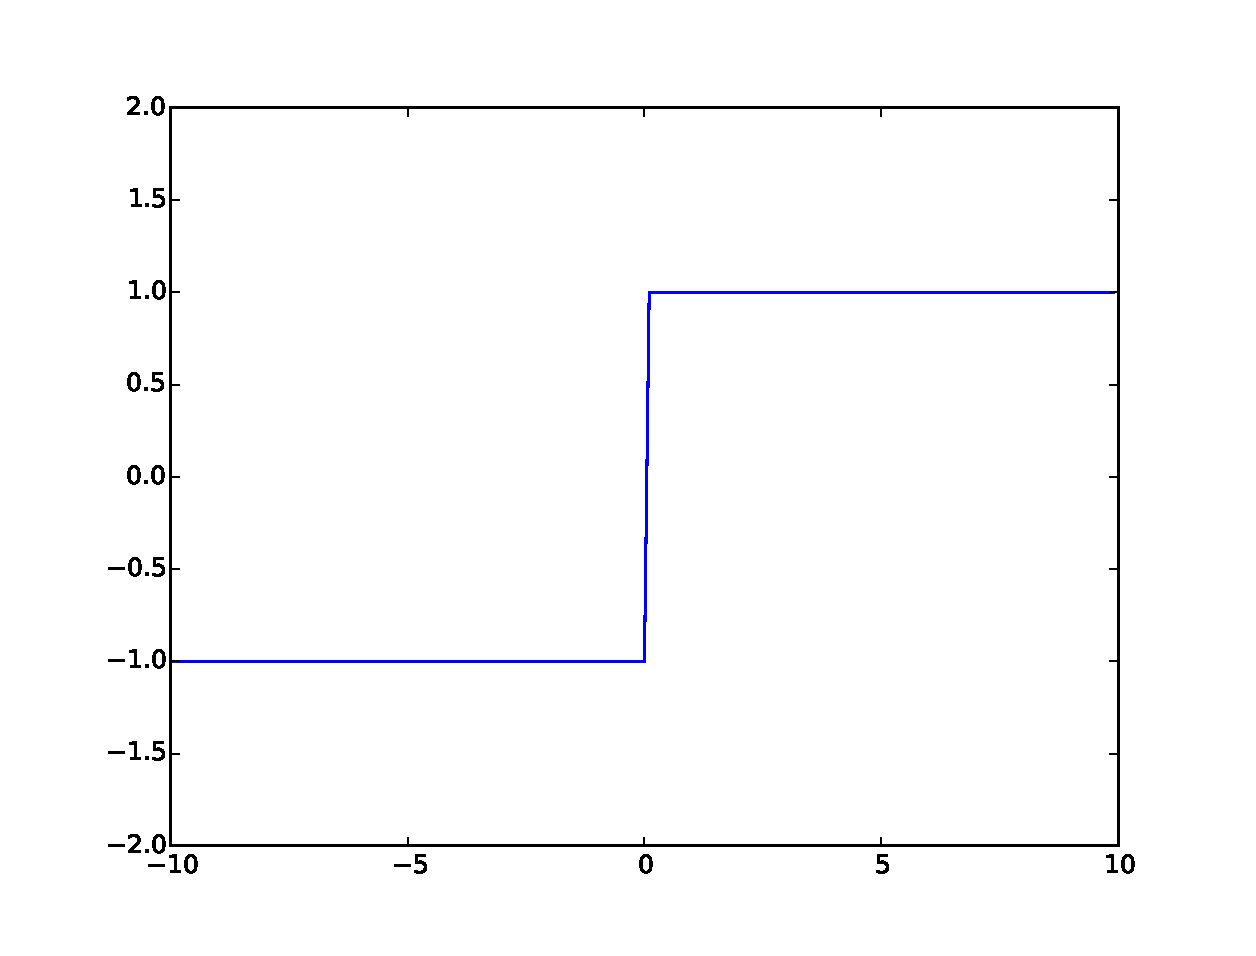
\includegraphics[height=4cm, width=6cm]{threshold.eps}
	\caption{デジタル出力モデル}
\end{figure}
\end{column}
\end{columns}
ゲインのスケールが大きければ大きいほど、出力の増加が急になる。 \\
デジタル出力モデルは、ゲインのスケールの極限として解釈できる。
\end{frame}

\begin{frame}\frametitle{ニューラルネットワークの分類}
大きく分けて2種類のネットワーク構造がある。
\begin{columns}[T]		
\begin{column}[T]{5cm}
\begin{figure}[htbp]
	\includegraphics[height=3.8cm, width=5.5cm]{feedforward_networks.png}
	\caption{フィードフォワード型}
\end{figure}
パターン認識(回帰、分類)
\end{column}
\begin{column}[T]{5cm}
\begin{figure}[htbp]
	\includegraphics[height=3.8cm, width=5.5cm]{feedback_networks}
	\caption{フィードバック型}
\end{figure}
連想記憶 \\
組み合わせ最適化
\end{column}
\end{columns}
\end{frame}

\begin{frame}\frametitle{ホップフィールド・ネットワークとは}
フィードバック型のニューラルネットワークのモデルの1種で、次の性質を持つものである。
\vspace{0.5cm}
\begin{enumerate}
\item[1] 対称的な相互作用をもつ
\item[2] 非同期的に状態を更新する
\end{enumerate}
\vspace{0.5cm}
自然な操作により、ネットワークのエネルギーが極小の状態に収束する。
\end{frame}

\begin{frame}\frametitle{巡回セールスマン問題(TSP)とは}
\begin{block}{巡回セールスマン問題(Traveling Salesman Problem)}
都市の集合と各2都市間の移動コストが与えられたとき、全ての都市をちょうど一度ずつ巡り出発地に戻る巡回路のうち、総移動コストが最小のものを求めよ。
\end{block}
\begin{center}
\includegraphics[height=4cm, width=6cm]{opt_route.eps}
\end{center}
都市の数$N$に対して、異なる長さを持つ経路が$\dfrac{N!}{2N}$通り存在する。
\end{frame}

\begin{frame}\frametitle{ニューラルネットワークによる巡回路の表現}
$i$番目に都市$X$に訪れることを、$V_{Xi} = 1$とする。(それ以外は$0$)
\begin{columns}[T]
\begin{column}[T]{5cm}
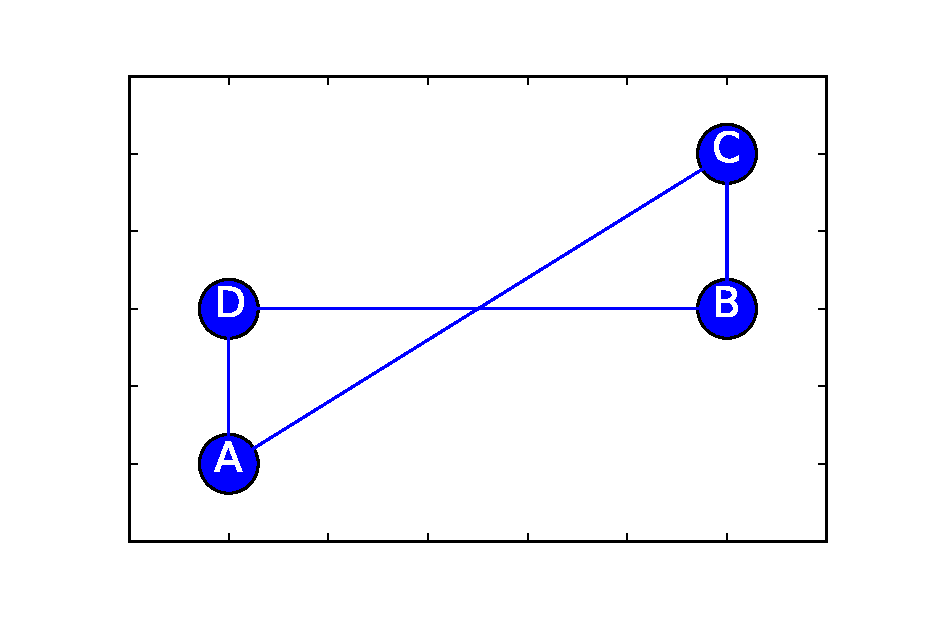
\includegraphics[height=5cm, width=6cm]{route.eps}
\end{column}
\begin{column}[T]{5cm}
\vspace{1cm}
\large{
\[
  \left(
    \begin{array}{cccc}
      1 & 0 & 0 & 0  \\
      0 & 0 & 1 & 0 \\
      0 & 0 & 0 & 1 \\
      0 & 1 & 0 & 0
    \end{array}
  \right)
\]
}
\end{column}
\end{columns}
このとき$N$都市の巡回路は、$N^{2}$個のニューロンからなる \\
$N \times N$の置換行列$\{V_{Xi}\}$で表現できる。\\
\end{frame}

\begin{frame}\frametitle{ニューラルネットによる解法の概要}
ホップフィールド・ネットワークの力学系では、力学系の安定点がエネルギー関数の極小点になる。\\
\vspace{1cm}
エネルギー関数の極小点と総移動コストが最小の巡回路を対応させることができれば、イテレーションによって解を求めることができる。
\end{frame}

\begin{frame}\frametitle{エネルギー関数への要請}
力学系の安定点が表す巡回路が
\vspace{0.5cm}
\begin{enumerate}
\item[1] 有効な巡回路を表す。(置換行列になっている)
\item[2] 総移動コストが小さい。
\end{enumerate}
\vspace{0.5cm}
という性質を満たすようにエネルギー関数を定義する。
\end{frame}

\begin{frame}\frametitle{エネルギー関数の性質1}
\begin{enumerate}
\item[1] 有効な巡回路を表す。 \\
\begin{equation}
	\label{equation:1}
	\displaystyle \frac{A}{2}\sum_{X}\sum_{i}\sum_{j \neq i} V_{Xi}V_{X_{j}}
    + \frac{B}{2}\sum_{i}\sum_{X}\sum_{Y \neq X} V_{Xi}V_{Yi}
    + \frac{C}{2}\sum_{X}\sum_{i}(V_{Xi} - n)^2    
\end{equation}
\end{enumerate}
ここで、$V_{Xi}$はニューロンの$(X, i)$成分、 $A, B, C$は定数である。 \\
\vspace{0.5cm}
各項は、次が成り立つときにのみ$0$となり、それ以外で正の値。
\begin{enumerate}
\item[(a)] 都市を1度だけ訪れる。
\item[(b)] 1度に訪れる都市は1つ。
\item[(c)] 全部で$n$回訪れる。
\end{enumerate}
\vspace{0.5cm}
\large{
したがって、(\ref{equation:1})全体で巡回路の有効性を表す。
}
\end{frame}

\begin{frame}\frametitle{エネルギー関数の性質2}
\begin{enumerate}
\item[2] 総移動コストが小さい。 \\
\begin{equation}
	\label{equation:2}
	\displaystyle \frac{D}{2} \sum_{X}\sum_{Y \neq X}\sum_{i} d_{XY}V_{Xi}(V_{Y, i+1} + V_{Y, i-1})
\end{equation}

\vspace{1cm}
ここで、$d_{XY}$は2都市$X, Y$間の移動コスト、$D$は定数である。 \\
\vspace{1.0cm}
(\ref{equation:2})は、$\{V_{Xi}\}$が置換行列のとき、総移動コストと一致する。
\end{enumerate}
\end{frame}

\begin{frame}\frametitle{エネルギー関数の定義}
エネルギー関数$E$を$(\ref{equation:1}) + (\ref{equation:2})$で定義する。
\begin{block}{エネルギー関数}
\begin{equation}
\label{eq:energy_function}
\begin{split}
	E &:= 	\displaystyle \frac{A}{2}\sum_{X}\sum_{i}\sum_{j \neq i} V_{Xi}V_{X_{j}}
    + \frac{B}{2}\sum_{i}\sum_{X}\sum_{Y \neq X} V_{Xi}V_{Yi} \\
    & \quad + \frac{C}{2}\sum_{X}\sum_{i}(V_{Xi} - n)^2 \\
    & \quad + \frac{D}{2} \sum_{X}\sum_{Y \neq X}\sum_{i} d_{XY}V_{Xi}(V_{Y, i+1} + V_{Y, i-1})
\end{split}
\end{equation}
\end{block}
\vspace{1cm}
定数$A, B, C$が大きいとき、巡回路の有効性は保証されるが、総移動コストが小さくならないことがある。\\
逆に、定数$D$が大きいとき、総移動コストが小さくなるが、巡回路の有効性が保証されない。
\end{frame}

\begin{frame}\frametitle{結合行列と外力}
エネルギー関数\eqref{eq:energy_function}を$V_{Xi}$で偏微分することにより、 結合行列$T_{XiYj}$($N^2 \times N^2$行列)と外力$I_{Xi}$が得られる。
\begin{block}{結合行列と外力}
\begin{equation}
\begin{split}
T_{XiYj} &= -A\delta_{XY}(1 - \delta_{ij}) \\
			& \quad -B\delta_{ij}(1 - \delta_{XY}) \\
            & \quad - C \\
            & \quad -Dd_{XY}(\delta_{j, i+1} + \delta_{j, i-1})
\end{split}
\end{equation}
\begin{equation}
I_{Xi} = +Cn
\end{equation}
\end{block}
\end{frame}

\begin{frame}\frametitle{運動方程式}
任意時刻の各ニューロンの出力$V_{Xi}$は、次の運動方程式によって決定する。
\begin{block}{運動方程式}
\begin{equation}
\begin{split}
	\displaystyle \frac{du_{Xi}}{dt} &= \frac{-u_{Xi}}{\tau} - A\sum_{j \neq i}V_{Xj} - B\sum_{Y \neq X}V_{Yi} \\
    & \quad -C(\sum_{X}\sum_{j}V_{Xj} - n) \\
    & \quad -D\sum_{Y}d_{XY}(V_{Y, i+1} + V_{Y, i-1})
\end{split}
\end{equation}
\begin{equation}
	V_{Xi} = sigmoid(u_{Xi}) = \displaystyle \frac{1}{2}(1 + tanh(\frac{u_{Xi}}{u_{0}}))
\end{equation}
\end{block}
一般性を失わずに、$\tau = 1$として良い。 \\
$u_{0}^{-1}$は、シグモイド関数のゲイン。
\end{frame}

\begin{comment}

\begin{frame}\frametitle{データセット}
TSPLIB \\
\url{(http://comopt.ifi.uni-heidelberg.de/software/TSPLIB95/)} \\
巡回セールスマン問題に関するデータセット。\\
\vspace{1cm}
都市の位置を表す二次元の点の集合と最適解である最小経路がセットになっている。
\end{frame}

\begin{frame}\frametitle{データの可視化}
22箇所の都市の場合
\vspace{-0.5cm}
\begin{columns}[T]		
\begin{column}[T]{5cm}
\begin{figure}[htbp]
	\includegraphics[height=5.5cm, width=6.5cm]{random_route.eps}
	\caption{適当な巡回路}
\end{figure}
\[ L \approx 132.489 \]
\end{column}
\begin{column}[T]{5cm}
\begin{figure}[htbp]
	\includegraphics[height=5.5cm, width=6.5cm]{opt_route.eps}
	\caption{最短の巡回路}
\end{figure}
\[ L \approx 75.665 \]
\end{column}
\end{columns}
\end{frame}

\begin{frame}\frametitle{データの観察}
ランダムに生成した巡回路1000個に対して、総移動コストを計算。
\begin{figure}[htbp]
\includegraphics[height=7cm, width=10cm]{hist.eps}
\caption{総移動コストの分布}
\end{figure}
\end{frame}

\end{comment}

\begin{frame}\frametitle{今後の課題}
\Large{
\begin{enumerate}
\item シミュレーティド・アニーリング(Sree Aiyer[1991])
\vspace{1.0cm}
\item ボルツマンマシン(確率的に出力を決定)
\vspace{1.0cm}
\item フィードバックに遅れの効果を入れる。
\vspace{1.0cm}
\item TSP以外の組み合わせ最適化問題への応用(暗号の解読、 グラフ分割問題etc)
\end{enumerate}
}
\end{frame}

\begin{frame}\frametitle{興味あること}
\Large{
\begin{enumerate}
\item 生物の挙動をモデル化して、シミュレーションすることで、知的な振る舞いを再現・応用すること。
\vspace{1.0cm}
\item 局所的で単純なルールだけから、全体として複雑な挙動を得ること(自己組織化)
\vspace{1.0cm}
\item 確率論的プログラミング(確率を用いて効率的に問題解決)
\end{enumerate}
}
\end{frame}

\begin{frame}\frametitle{参考文献}
\begin{enumerate}
\item[1] J. J. Hopfield D. W. Tank, “Neural” computation of decisions in optimization problems, 1985 
\end{enumerate}
\end{frame}

\end{document}